\section{Simple function task}
\subsection{Dataset generation}
\label{sec:appendix:simple-function-task:data-generation}

\begin{figure}[h]
\centering
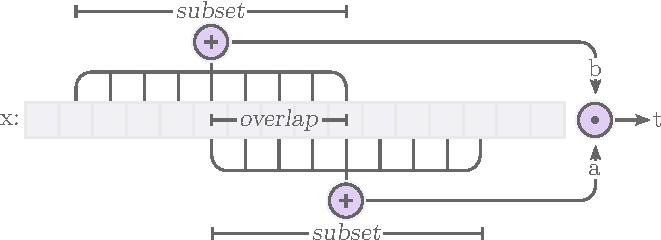
\includegraphics[scale=0.8]{graphics/function_task_static_problem.pdf}
\caption{Dataset is parameterized into ``Input Size'', ``Subset Ratio'', ``Overlap Ratio'', an Operation (here showing multiplication), ``Interpolation Range'' and ``Extrapolation Range'' from which the data set sampled.}
\label{fig:simple-function-task-problem}
\end{figure}

All datasets in the simple function task experiments are generated using algorithm \ref{alg:dataset-sampling}. Its parameters are visualized in figure \ref{fig:simple-function-task-problem}.

\begin{algorithm}[h]
  \caption{Dataset sampling algorithm}
  \begin{algorithmic}[1]
    \Function{Dataset}{${\Call{Op}{\cdot, \cdot}: \mathrm{Operation}}$, ${i: \mathrm{Input Size}}$, ${s: \mathrm{Subset Ratio}}$, ${o: \mathrm{Overlap Ratio}}$, ${\hspace{3cm}R: \mathrm{Range}}$}
      \Let{$\mathbf{x}$}{\Call{Uniform}{$R_{lower}, R_{upper}, i$}} \Comment{Sample $i$ elements uniformly}
      \Let{$k$}{\Call{Uniform}{$0, 1 - 2s - o$}} \Comment{Sample offset}
      \Let{$a$}{\Call{Sum}{$\mathbf{x}[ik:i(k+s)]$}} \Comment{Create sum $a$ from subset}
      \Let{$b$}{\Call{Sum}{$\mathbf{x}[i(k+s-o):i (k+2s-0)]$}} \Comment{Create sum $b$ from subset}
      \Let{$t$}{\Call{Op}{$a, b$}} \Comment{Perform operation on $a$ and $b$}
      \State \Return{$x, t$}
    \EndFunction
  \end{algorithmic}
  \label{alg:dataset-sampling}
\end{algorithm}

\subsection{Arithmetic operations comparison - all models}

\begin{table}[h]
\caption{Model definitions}
\label{tab:model-defintions}
\centering
\begin{tabular}{r l l}
\toprule
 Model & Layer 1 & Layer 2 \\
 \midrule
 NMU & NAU & NMU \\
 NAU & NAU & NAU \\
 $\mathrm{NAC}_{\bullet}$ & $\mathrm{NAC}_{+}$ & $\mathrm{NAC}_{\bullet}$ \\
 $\mathrm{NAC}_{+}$ & $\mathrm{NAC}_{+}$ & $\mathrm{NAC}_{+}$ \\
 NALU & NALU & NALU \\
 Linear & Linear & Linear \\
 ReLU & ReLU & ReLU \\
 ReLU6 & ReLU6 & ReLU6 \\
 \bottomrule
\end{tabular}
\end{table}

Results for all models on addition, subtraction, and multiplication can be found in table \ref{tab:function-task-static-defaults-all}.

\label{sec:appendix:function-task-static-all-comparision}

\begin{longtable}{crllll}
\caption{\label{tab:function-task-static-defaults-all}Shows the success-rate, when the model converged, and the sparsity error for all weight matrices, with 95\% confidence interval. Each value is a summary of 100 different seeds.}\\
\toprule
\multicolumn{1}{c}{Op} & \multicolumn{1}{c}{Model} & \multicolumn{1}{c}{Success} & \multicolumn{2}{c}{Solved at} & \multicolumn{1}{c}{Sparsity error} \\
\cmidrule(l{3pt}r{3pt}){1-1} \cmidrule(l{3pt}r{3pt}){2-2} \cmidrule(l{3pt}r{3pt}){3-3} \cmidrule(l{3pt}r{3pt}){4-5} \cmidrule(l{3pt}r{3pt}){6-6}
 &  & Rate & Median & Mean & Mean\\
\midrule
\endfirsthead
\caption[]{Shows the success-rate, when the model converged, and the sparsity error for all weight matrices, with 95\% confidence interval. Each value is a summary of 100 different seeds. \textit{(continued)}}\\
\toprule
\multicolumn{1}{c}{Op} & \multicolumn{1}{c}{Model} & \multicolumn{1}{c}{Success} & \multicolumn{2}{c}{Solved at} & \multicolumn{1}{c}{Sparsity error} \\
\cmidrule(l{3pt}r{3pt}){1-1} \cmidrule(l{3pt}r{3pt}){2-2} \cmidrule(l{3pt}r{3pt}){3-3} \cmidrule(l{3pt}r{3pt}){4-5} \cmidrule(l{3pt}r{3pt}){6-6}
 &  & Rate & Median & Mean & Mean\\
\midrule
\endhead
\
\endfoot
\bottomrule
\endlastfoot
 & $\mathrm{NAC}_{\bullet,\mathrm{NMU}}$ & $93\% {~}^{+4\%}_{-7\%}$ & $1.8 \cdot 10^{6}$ & $1.9 \cdot 10^{6} {~}^{+7.7 \cdot 10^{4}}_{-9.3 \cdot 10^{4}}$ & $9.5 \cdot 10^{-7} {~}^{+4.2 \cdot 10^{-7}}_{-4.2 \cdot 10^{-7}}$\\

\nopagebreak
 & $\mathrm{NAC}_{\bullet,\sigma}$ & $\mathbf{100\%} {~}^{+0\%}_{-4\%}$ & $2.5 \cdot 10^{6}$ & $2.6 \cdot 10^{6} {~}^{+8.8 \cdot 10^{4}}_{-7.2 \cdot 10^{4}}$ & $4.6 \cdot 10^{-5} {~}^{+5.0 \cdot 10^{-6}}_{-5.6 \cdot 10^{-6}}$\\

\nopagebreak
 & $\mathrm{NAC}_{\bullet}$ & $31\% {~}^{+10\%}_{-8\%}$ & $2.8 \cdot 10^{6}$ & $3.0 \cdot 10^{6} {~}^{+2.9 \cdot 10^{5}}_{-2.4 \cdot 10^{5}}$ & $5.8 \cdot 10^{-4} {~}^{+4.8 \cdot 10^{-4}}_{-2.6 \cdot 10^{-4}}$\\

\nopagebreak
 & $\mathrm{NAC}_{+}$ & $0\% {~}^{+4\%}_{-0\%}$ & --- & --- & ---\\

\nopagebreak
 & Linear & $0\% {~}^{+4\%}_{-0\%}$ & --- & --- & ---\\

\nopagebreak
 & NALU & $0\% {~}^{+4\%}_{-0\%}$ & --- & --- & ---\\

\nopagebreak
 & NAU & $0\% {~}^{+4\%}_{-0\%}$ & --- & --- & ---\\

\nopagebreak
 & NMU & $98\% {~}^{+1\%}_{-5\%}$ & $\mathbf{1.4 \cdot 10^{6}}$ & $\mathbf{1.5 \cdot 10^{6}} {~}^{+4.8 \cdot 10^{4}}_{-6.5 \cdot 10^{4}}$ & $\mathbf{4.2 \cdot 10^{-7}} {~}^{+2.9 \cdot 10^{-8}}_{-2.9 \cdot 10^{-8}}$\\

\nopagebreak
 & ReLU & $0\% {~}^{+4\%}_{-0\%}$ & --- & --- & ---\\

\nopagebreak
\multirow{-10}{*}{\centering\arraybackslash $\bm{\times}$} & ReLU6 & $0\% {~}^{+4\%}_{-0\%}$ & --- & --- & ---\\
\cmidrule{1-6}
 & $\mathrm{NAC}_{\bullet,\mathrm{NMU}}$ & $\mathbf{0\%} {~}^{+4\%}_{-0\%}$ & --- & --- & ---\\

\nopagebreak
 & $\mathrm{NAC}_{\bullet,\sigma}$ & $\mathbf{0\%} {~}^{+4\%}_{-0\%}$ & --- & --- & ---\\

\nopagebreak
 & $\mathrm{NAC}_{\bullet}$ & $\mathbf{0\%} {~}^{+4\%}_{-0\%}$ & --- & --- & ---\\

\nopagebreak
 & $\mathrm{NAC}_{+}$ & $\mathbf{0\%} {~}^{+4\%}_{-0\%}$ & --- & --- & ---\\

\nopagebreak
 & Linear & $\mathbf{0\%} {~}^{+4\%}_{-0\%}$ & --- & --- & ---\\

\nopagebreak
 & NALU & $\mathbf{0\%} {~}^{+4\%}_{-0\%}$ & --- & --- & ---\\

\nopagebreak
 & NAU & $\mathbf{0\%} {~}^{+4\%}_{-0\%}$ & --- & --- & ---\\

\nopagebreak
 & NMU & $\mathbf{0\%} {~}^{+4\%}_{-0\%}$ & --- & --- & ---\\

\nopagebreak
 & ReLU & $\mathbf{0\%} {~}^{+4\%}_{-0\%}$ & --- & --- & ---\\

\nopagebreak
\multirow{-10}{*}{\centering\arraybackslash $\bm{\mathbin{/}}$} & ReLU6 & $\mathbf{0\%} {~}^{+4\%}_{-0\%}$ & --- & --- & ---\\
\cmidrule{1-6}
 & $\mathrm{NAC}_{\bullet,\mathrm{NMU}}$ & $0\% {~}^{+4\%}_{-0\%}$ & --- & --- & ---\\

\nopagebreak
 & $\mathrm{NAC}_{\bullet,\sigma}$ & $0\% {~}^{+4\%}_{-0\%}$ & --- & --- & ---\\

\nopagebreak
 & $\mathrm{NAC}_{\bullet}$ & $0\% {~}^{+4\%}_{-0\%}$ & --- & --- & ---\\

\nopagebreak
 & $\mathrm{NAC}_{+}$ & $\mathbf{100\%} {~}^{+0\%}_{-4\%}$ & $2.5 \cdot 10^{5}$ & $4.9 \cdot 10^{5} {~}^{+5.2 \cdot 10^{4}}_{-4.5 \cdot 10^{4}}$ & $2.3 \cdot 10^{-1} {~}^{+6.5 \cdot 10^{-3}}_{-6.5 \cdot 10^{-3}}$\\

\nopagebreak
 & Linear & $\mathbf{100\%} {~}^{+0\%}_{-4\%}$ & $6.1 \cdot 10^{4}$ & $\mathbf{6.3 \cdot 10^{4}} {~}^{+2.5 \cdot 10^{3}}_{-3.3 \cdot 10^{3}}$ & $2.5 \cdot 10^{-1} {~}^{+3.6 \cdot 10^{-4}}_{-3.6 \cdot 10^{-4}}$\\

\nopagebreak
 & NALU & $14\% {~}^{+8\%}_{-5\%}$ & $1.5 \cdot 10^{6}$ & $1.6 \cdot 10^{6} {~}^{+3.8 \cdot 10^{5}}_{-3.3 \cdot 10^{5}}$ & $1.7 \cdot 10^{-1} {~}^{+2.7 \cdot 10^{-2}}_{-2.5 \cdot 10^{-2}}$\\

\nopagebreak
 & NAU & $\mathbf{100\%} {~}^{+0\%}_{-4\%}$ & $\mathbf{1.8 \cdot 10^{4}}$ & $3.9 \cdot 10^{5} {~}^{+4.4 \cdot 10^{4}}_{-3.7 \cdot 10^{4}}$ & $\mathbf{3.2 \cdot 10^{-5}} {~}^{+1.3 \cdot 10^{-5}}_{-1.3 \cdot 10^{-5}}$\\

\nopagebreak
 & NMU & $0\% {~}^{+4\%}_{-0\%}$ & --- & --- & ---\\

\nopagebreak
 & ReLU & $62\% {~}^{+9\%}_{-10\%}$ & $6.2 \cdot 10^{4}$ & $7.6 \cdot 10^{4} {~}^{+8.3 \cdot 10^{3}}_{-7.0 \cdot 10^{3}}$ & $2.5 \cdot 10^{-1} {~}^{+2.4 \cdot 10^{-3}}_{-2.4 \cdot 10^{-3}}$\\

\nopagebreak
\multirow{-10}{*}{\centering\arraybackslash $\bm{+}$} & ReLU6 & $0\% {~}^{+4\%}_{-0\%}$ & --- & --- & ---\\
\cmidrule{1-6}
 & $\mathrm{NAC}_{\bullet,\mathrm{NMU}}$ & $0\% {~}^{+4\%}_{-0\%}$ & --- & --- & ---\\

\nopagebreak
 & $\mathrm{NAC}_{\bullet,\sigma}$ & $0\% {~}^{+4\%}_{-0\%}$ & --- & --- & ---\\

\nopagebreak
 & $\mathrm{NAC}_{\bullet}$ & $0\% {~}^{+4\%}_{-0\%}$ & --- & --- & ---\\

\nopagebreak
 & $\mathrm{NAC}_{+}$ & $\mathbf{100\%} {~}^{+0\%}_{-4\%}$ & $9.0 \cdot 10^{3}$ & $3.7 \cdot 10^{5} {~}^{+3.8 \cdot 10^{4}}_{-3.8 \cdot 10^{4}}$ & $2.3 \cdot 10^{-1} {~}^{+5.4 \cdot 10^{-3}}_{-5.4 \cdot 10^{-3}}$\\

\nopagebreak
 & Linear & $7\% {~}^{+7\%}_{-4\%}$ & $3.3 \cdot 10^{6}$ & $1.4 \cdot 10^{6} {~}^{+7.0 \cdot 10^{5}}_{-6.1 \cdot 10^{5}}$ & $1.8 \cdot 10^{-1} {~}^{+7.2 \cdot 10^{-2}}_{-5.8 \cdot 10^{-2}}$\\

\nopagebreak
 & NALU & $14\% {~}^{+8\%}_{-5\%}$ & $1.9 \cdot 10^{6}$ & $1.9 \cdot 10^{6} {~}^{+4.4 \cdot 10^{5}}_{-4.5 \cdot 10^{5}}$ & $2.1 \cdot 10^{-1} {~}^{+2.2 \cdot 10^{-2}}_{-2.2 \cdot 10^{-2}}$\\

\nopagebreak
 & NAU & $\mathbf{100\%} {~}^{+0\%}_{-4\%}$ & $\mathbf{5.0 \cdot 10^{3}}$ & $\mathbf{1.6 \cdot 10^{5}} {~}^{+1.7 \cdot 10^{4}}_{-1.6 \cdot 10^{4}}$ & $6.6 \cdot 10^{-2} {~}^{+2.5 \cdot 10^{-2}}_{-1.9 \cdot 10^{-2}}$\\

\nopagebreak
 & NMU & $56\% {~}^{+9\%}_{-10\%}$ & $1.0 \cdot 10^{6}$ & $1.0 \cdot 10^{6} {~}^{+5.8 \cdot 10^{2}}_{-5.8 \cdot 10^{2}}$ & $\mathbf{3.4 \cdot 10^{-4}} {~}^{+3.2 \cdot 10^{-5}}_{-2.6 \cdot 10^{-5}}$\\

\nopagebreak
 & ReLU & $0\% {~}^{+4\%}_{-0\%}$ & --- & --- & ---\\

\nopagebreak
\multirow{-10}{*}{\centering\arraybackslash $\bm{-}$} & ReLU6 & $0\% {~}^{+4\%}_{-0\%}$ & --- & --- & ---\\
\cmidrule{1-6}
 & $\mathrm{NAC}_{\bullet,\mathrm{NMU}}$ & $3\% {~}^{+5\%}_{-2\%}$ & $1.0 \cdot 10^{6}$ & $\mathbf{1.0 \cdot 10^{6}}$ & $\mathbf{1.7 \cdot 10^{-1}} {~}^{+8.3 \cdot 10^{-3}}_{-8.1 \cdot 10^{-3}}$\\

\nopagebreak
 & $\mathrm{NAC}_{\bullet,\sigma}$ & $0\% {~}^{+4\%}_{-0\%}$ & --- & --- & ---\\

\nopagebreak
 & $\mathrm{NAC}_{\bullet}$ & $\mathbf{7\%} {~}^{+7\%}_{-4\%}$ & $\mathbf{4.0 \cdot 10^{5}}$ & $1.5 \cdot 10^{6} {~}^{+6.0 \cdot 10^{5}}_{-5.6 \cdot 10^{5}}$ & $2.4 \cdot 10^{-1} {~}^{+1.7 \cdot 10^{-2}}_{-1.7 \cdot 10^{-2}}$\\

\nopagebreak
 & $\mathrm{NAC}_{+}$ & $0\% {~}^{+4\%}_{-0\%}$ & --- & --- & ---\\

\nopagebreak
 & Linear & $0\% {~}^{+4\%}_{-0\%}$ & --- & --- & ---\\

\nopagebreak
 & NALU & $2\% {~}^{+5\%}_{-1\%}$ & $2.6 \cdot 10^{6}$ & $3.3 \cdot 10^{6} {~}^{+1.8 \cdot 10^{6}}_{-2.2 \cdot 10^{6}}$ & $5.0 \cdot 10^{-1} {~}^{+2.5 \cdot 10^{-6}}_{-8.0 \cdot 10^{-6}}$\\

\nopagebreak
 & NAU & $0\% {~}^{+4\%}_{-0\%}$ & --- & --- & ---\\

\nopagebreak
 & NMU & $0\% {~}^{+4\%}_{-0\%}$ & --- & --- & ---\\

\nopagebreak
 & ReLU & $0\% {~}^{+4\%}_{-0\%}$ & --- & --- & ---\\

\nopagebreak
\multirow{-10}{*}{\centering\arraybackslash $\sqrt{z}$} & ReLU6 & $0\% {~}^{+4\%}_{-0\%}$ & --- & --- & ---\\
\cmidrule{1-6}
 & $\mathrm{NAC}_{\bullet,\mathrm{NMU}}$ & $\mathbf{100\%} {~}^{+0\%}_{-4\%}$ & $1.4 \cdot 10^{6}$ & $1.5 \cdot 10^{6} {~}^{+7.1 \cdot 10^{4}}_{-5.9 \cdot 10^{4}}$ & $\mathbf{2.9 \cdot 10^{-7}} {~}^{+1.4 \cdot 10^{-8}}_{-1.4 \cdot 10^{-8}}$\\

\nopagebreak
 & $\mathrm{NAC}_{\bullet,\sigma}$ & $\mathbf{100\%} {~}^{+0\%}_{-4\%}$ & $1.9 \cdot 10^{6}$ & $1.9 \cdot 10^{6} {~}^{+5.3 \cdot 10^{4}}_{-6.2 \cdot 10^{4}}$ & $1.8 \cdot 10^{-2} {~}^{+4.3 \cdot 10^{-4}}_{-4.3 \cdot 10^{-4}}$\\

\nopagebreak
 & $\mathrm{NAC}_{\bullet}$ & $77\% {~}^{+7\%}_{-9\%}$ & $3.3 \cdot 10^{6}$ & $3.2 \cdot 10^{6} {~}^{+1.6 \cdot 10^{5}}_{-2.0 \cdot 10^{5}}$ & $1.8 \cdot 10^{-2} {~}^{+5.8 \cdot 10^{-4}}_{-5.7 \cdot 10^{-4}}$\\

\nopagebreak
 & $\mathrm{NAC}_{+}$ & $0\% {~}^{+4\%}_{-0\%}$ & --- & --- & ---\\

\nopagebreak
 & Linear & $0\% {~}^{+4\%}_{-0\%}$ & --- & --- & ---\\

\nopagebreak
 & NALU & $0\% {~}^{+4\%}_{-0\%}$ & --- & --- & ---\\

\nopagebreak
 & NAU & $0\% {~}^{+4\%}_{-0\%}$ & --- & --- & ---\\

\nopagebreak
 & NMU & $\mathbf{100\%} {~}^{+0\%}_{-4\%}$ & $\mathbf{1.2 \cdot 10^{6}}$ & $\mathbf{1.3 \cdot 10^{6}} {~}^{+3.1 \cdot 10^{4}}_{-3.6 \cdot 10^{4}}$ & $3.7 \cdot 10^{-5} {~}^{+5.4 \cdot 10^{-5}}_{-3.7 \cdot 10^{-5}}$\\

\nopagebreak
 & ReLU & $0\% {~}^{+4\%}_{-0\%}$ & --- & --- & ---\\

\nopagebreak
\multirow{-10}{*}{\centering\arraybackslash $z^2$} & ReLU6 & $0\% {~}^{+4\%}_{-0\%}$ & --- & --- & ---\\*
\end{longtable}


\subsection{Ablation study}
To validate our model, we perform an ablation on the multiplication problem.

Our ablation study (table \ref{tab:function-task-static-ablation}) show that regularization have little effect in terms of success rate. As it is analytically known that there is no gradient outside of $w \in [0,1]$ for the NMU, the conclusion must be that the optimal weight initialization for the default dataset parameters and tested seeds, does not cause any weights to accidentally break out of $w \in [0,1]$. The sparse regularizer for multiplication have no sparsity effect, as only a sparse solution is a valid solution for multiplication. Although as seen in appendix \ref{sec:appendix:simple-function-task:regualization}, sparsity regularization can improve convergence.
\begin{table}[H]

\caption{\label{tab:function-task-static-ablation}Shows the success-rate for $\mathcal{L}_{\mathbf{W}_1, \mathbf{W}_2} < \mathcal{L}_{\mathbf{W}_1^\epsilon, \mathbf{W}_2^*}$, at what global step the model converged at, and the sparsity error for all weight matrices.}
\centering
\begin{tabular}{rllll}
\toprule
\multicolumn{1}{c}{Model} & \multicolumn{1}{c}{Success} & \multicolumn{2}{c}{Solved at} & \multicolumn{1}{c}{Sparsity error} \\
\cmidrule(l{3pt}r{3pt}){1-1} \cmidrule(l{3pt}r{3pt}){2-2} \cmidrule(l{3pt}r{3pt}){3-4} \cmidrule(l{3pt}r{3pt}){5-5}
 & Rate & Median & Mean & Mean\\
\midrule
$\mathrm{NAC}_{\bullet}$ & $40\%$ & $2.8 \cdot 10^{6}$ & $3.1 \cdot 10^{6} \pm 2.0 \cdot 10^{6}$ & $2.8 \cdot 10^{-2} \pm 8.9 \cdot 10^{-2}$\\

$\mathrm{NAC}_{\bullet}$, $\mathbf{W} = \sigma(\mathbf{\hat{W}})$ & $100\%$ & $1.9 \cdot 10^{6}$ & $1.9 \cdot 10^{6} \pm 3.1 \cdot 10^{5}$ & $1.1 \cdot 10^{-4} \pm 1.0 \cdot 10^{-4}$\\

NMU & $100\%$ & $1.2 \cdot 10^{6}$ & $1.2 \cdot 10^{6} \pm 2.0 \cdot 10^{5}$ & $1.6 \cdot 10^{-3} \pm 9.2 \cdot 10^{-4}$\\

NMU, $\mathbf{W} = \mathbf{\hat{W}}$ & $100\%$ & $1.3 \cdot 10^{6}$ & $1.2 \cdot 10^{6} \pm 1.9 \cdot 10^{5}$ & $3.9 \cdot 10^{-3} \pm 1.2 \cdot 10^{-3}$\\

NMU, $\mathbf{z} = \mathbf{W} \odot \mathbf{x}$ & $100\%$ & $1.2 \cdot 10^{6}$ & $1.2 \cdot 10^{6} \pm 2.0 \cdot 10^{5}$ & $1.6 \cdot 10^{-3} \pm 9.2 \cdot 10^{-4}$\\

NMU, no $\mathcal{R}_{oob}$ & $100\%$ & $1.2 \cdot 10^{6}$ & $1.2 \cdot 10^{6} \pm 1.9 \cdot 10^{5}$ & $1.7 \cdot 10^{-3} \pm 4.6 \cdot 10^{-4}$\\

NMU, no $\mathcal{R}_{sparse},\mathcal{R}_{oob}$ & $100\%$ & $1.1 \cdot 10^{6}$ & $1.1 \cdot 10^{6} \pm 1.8 \cdot 10^{5}$ & $3.3 \cdot 10^{-4} \pm 4.5 \cdot 10^{-5}$\\

NMU, no $\mathcal{R}_{sparse}$ & $100\%$ & $1.2 \cdot 10^{6}$ & $1.2 \cdot 10^{6} \pm 1.9 \cdot 10^{5}$ & $1.7 \cdot 10^{-3} \pm 9.0 \cdot 10^{-4}$\\
\bottomrule
\end{tabular}
\end{table}


Not allowing a multiplicative identity ($\mathbf{z} = \mathbf{W} \odot \mathbf{x}$), works when there is only two hidden units in the multiplication layer, as no multiplicative identity is necessary. However, for larger a hidden size as seen in figure \ref{fig:simple-function-static-ablation-hidden-size} identity becomes necessary.
\begin{figure}[h]
\centering
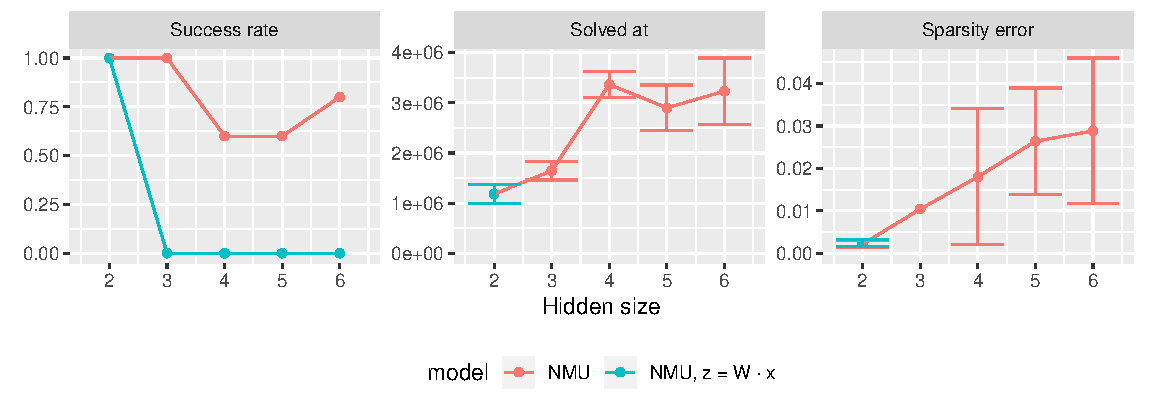
\includegraphics[width=\linewidth]{results/simple_function_static_ablation_hidden_size.pdf}
\caption{Compares NMU with NMU without identity, with different input size (hidden layer unit size) to the multiplication layer.}
\label{fig:simple-function-static-ablation-hidden-size}
\end{figure}

\clearpage
\subsection{Regularization}
\label{sec:appendix:simple-function-task:regualization}
A high sparsity regularization constant can help the model to converge faster. However, a regularization constant too high have have the inverse effect as well, or even make it impossible for the model to converge.
regularizer
In these experiments, the constant $c$ in equation \ref{eq:regualizer-experiment} is varied. See results in figure \ref{fig:simple-fnction-static-regularizer-add}, \ref{fig:simple-fnction-static-regularizer-sub}, and \ref{fig:simple-fnction-static-regularizer-mul}.
\begin{equation}
\lambda_{\mathrm{bias}} = c \cdot (1 - \exp(-10^5 \cdot t))
\label{eq:regualizer-experiment}
\end{equation}

\begin{figure}[h]
\centering
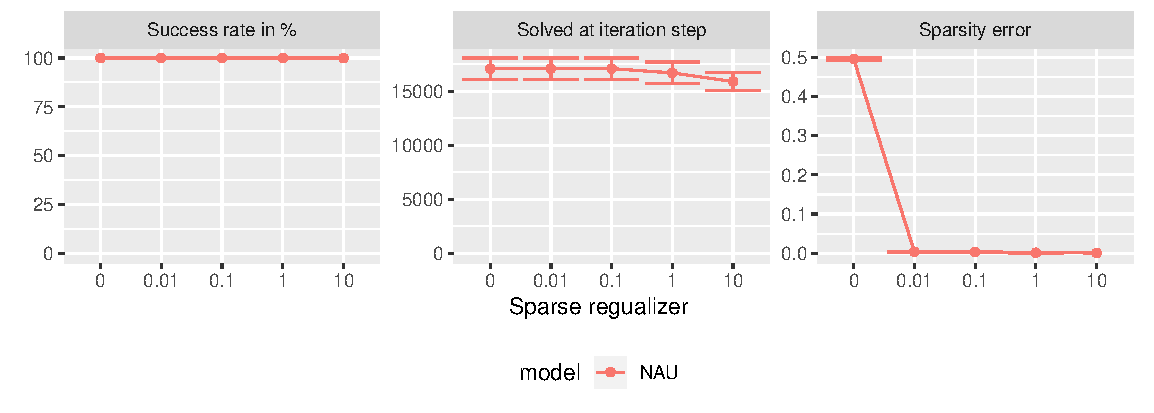
\includegraphics[width=\linewidth]{results/simple_function_static_regualization_add.pdf}
\caption{Shows the effect of the regularizer $\lambda_{\mathrm{bias}}$, on the simple function task problem for the $\bm{+}$ operation.}
\label{fig:simple-fnction-static-regularizer-add}
\end{figure}

\begin{figure}[h]
\centering
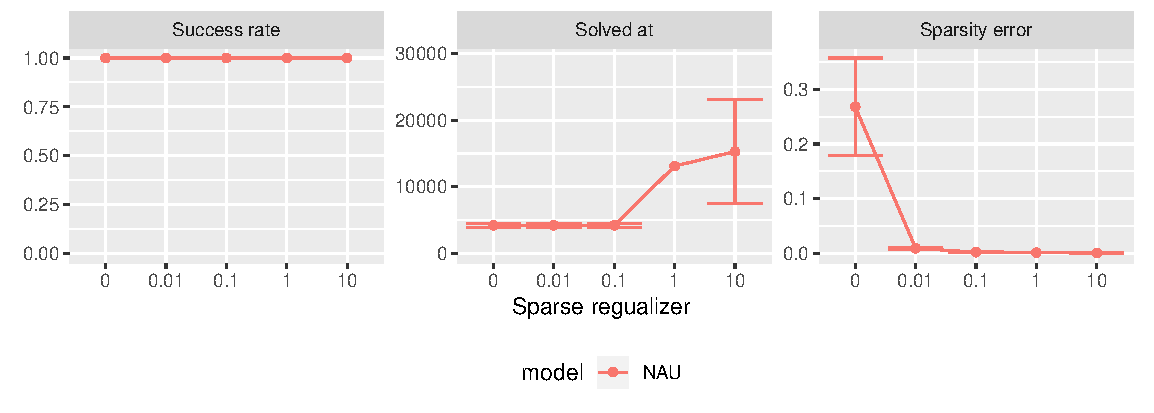
\includegraphics[width=\linewidth]{results/simple_function_static_regualization_sub.pdf}
\caption{Shows the effect of the regularizer $\lambda_{\mathrm{bias}}$, on the simple function task problem for the $\bm{-}$ operation.}
\label{fig:simple-fnction-static-regularizer-sub}
\end{figure}

\begin{figure}[h]
\centering
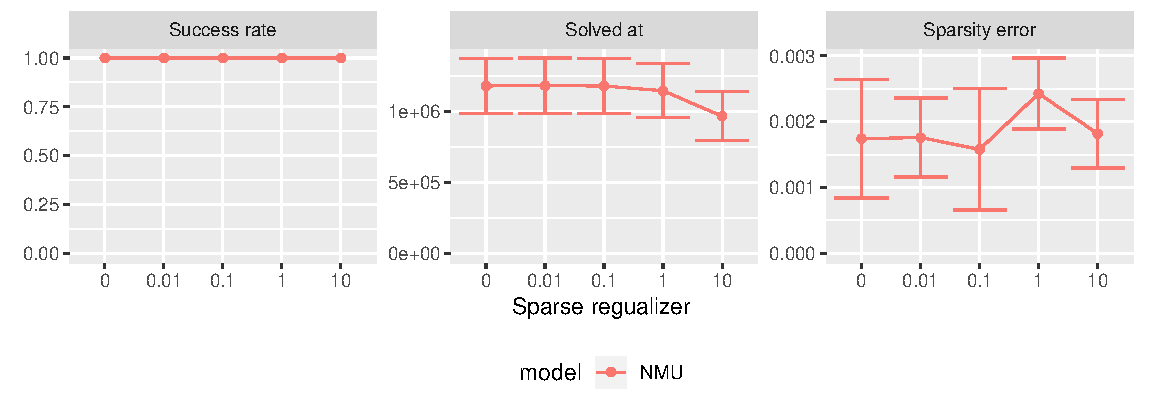
\includegraphics[width=\linewidth]{results/simple_function_static_regualization_mul.pdf}
\caption{Shows the effect of the regularizer $\lambda_{\mathrm{bias}}$, on the simple function task problem for the $\bm{\times}$ operation.}
\label{fig:simple-fnction-static-regularizer-mul}
\end{figure}

